% answers.tex —— 1997 年·全国卷·理科 · 参考答案与详细解析片段
% 由 tools/generate_projects.py 依来源总账自 1997/1997_数学真题_全国理_试题.md + 1997/1997_数学真题_全国理_解析正文.md + 1997/1997_数学真题_全国理_答案要点.md 生成，勿手改（改源 MD 后重跑）


\begin{gktip}
固定源 PDF 只有一页题面，没有答案和解析页。以下各题均依据题面独立推导；第 3、23 题的图形在 LaTeX 工程中以 TikZ 矢量源重绘。
\end{gktip}

\begin{answer}
\gksolhead{1}{}

\textbf{题目}：

\Needspace{5\baselineskip}
设集合

\nopagebreak[4]
\[
M=\{x\mid 0\leqslant x<2\},\qquad
N=\{x\mid x^2-2x-3<0\},
\]

集合 $M\cap N=$\mbox{（　　）}

（A）$\{x\mid 0\leqslant x<1\}$　　（B）$\{x\mid 0\leqslant x<2\}$

（C）$\{x\mid 0\leqslant x\leqslant 1\}$　　（D）$\{x\mid 0\leqslant x\leqslant 2\}$

\Needspace{4\baselineskip}
\textbf{解析}

\Needspace{5\baselineskip}
由

\nopagebreak[4]
\[
x^2-2x-3=(x+1)(x-3)
\]

\Needspace{5\baselineskip}
可知

\nopagebreak[4]
\[
N=\{x\mid -1<x<3\}.
\]

\Needspace{5\baselineskip}
与 $M=\{x\mid0\leqslant x<2\}$ 相交，得到

\nopagebreak[4]
\[
M\cap N=\{x\mid0\leqslant x<2\}.
\]

因此选 B。

\gkanswer{答案：B}

\end{answer}
\begin{answer}
\gksolhead{2}{}

\textbf{题目}：

如果直线 $ax+2y+2=0$ 与直线 $3x-y-2=0$ 平行，那么系数 $a=$\mbox{（　　）}

（A）$-3$　　（B）$-6$　　（C）$-\dfrac32$　　（D）$\dfrac23$

\Needspace{4\baselineskip}
\textbf{解析}

\Needspace{5\baselineskip}
两条直线的斜率分别为 $-a/2$ 和 $3$。平行时

\nopagebreak[4]
\[
-\frac a2=3,
\]

所以 $a=-6$，选 B。

\gkanswer{答案：B}

\end{answer}
\begin{answer}
\gksolhead{3}{}

\textbf{题目}：

\Needspace{5\baselineskip}
函数

\nopagebreak[4]
\[
y=\tan\left(\dfrac12x-\dfrac\pi3\right)
\]

在一个周期内的图象是\mbox{（　　）}
\nopagebreak[4]
\begin{center}% 1997 年全国卷理科第 3 题：四个正切函数图象选项
% 仅保留 TikZ/PGFPlots 矢量源；题面中的逻辑 PNG 标记不对应仓库文件。
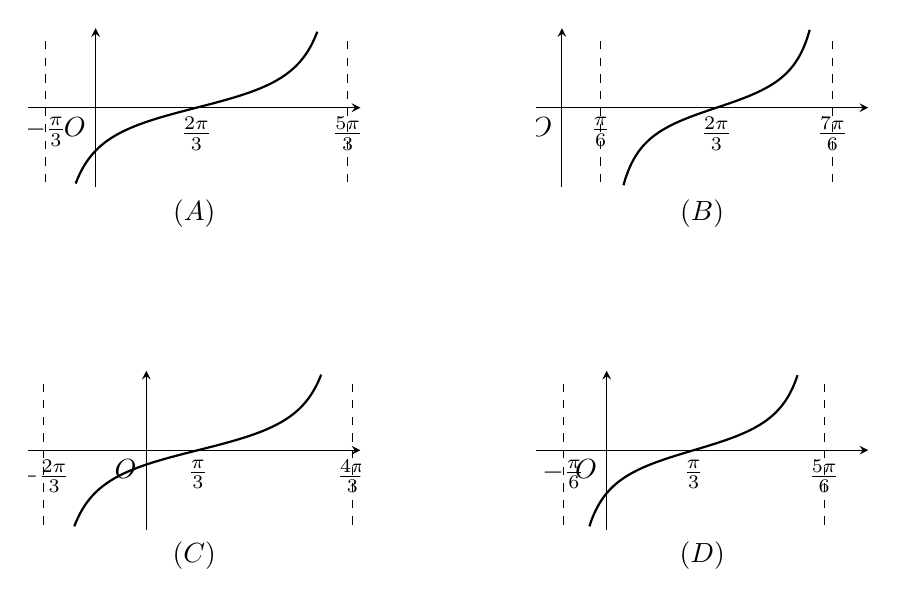
\begin{tikzpicture}[>=stealth]
  % (A)
  \begin{axis}[
    width=5.8cm, height=3.6cm,
    axis lines=middle, xmin=-1.4, xmax=5.5, ymin=-3.2, ymax=3.2,
    xtick=\empty, ytick=\empty, samples=240,
    restrict y to domain=-3.15:3.15, unbounded coords=jump,
    clip=true, title={$(A)$},
    title style={at={(axis description cs:0.5,-0.12)}, anchor=north},
  ]
    \addplot[thick, domain=-0.98:5.17]
      {tan(deg(0.5*x-pi/3))};
    \draw[dashed] (axis cs:-1.047,-3)--(axis cs:-1.047,3)
      (axis cs:5.236,-3)--(axis cs:5.236,3);
    \node[below] at (axis cs:-1.047,0) {$-\frac\pi3$};
    \node[below] at (axis cs:2.094,0) {$\frac{2\pi}3$};
    \node[below] at (axis cs:5.236,0) {$\frac{5\pi}3$};
    \node[below left] at (axis cs:0,0) {$O$};
  \end{axis}

  % (B)
  \begin{axis}[
    at={(6.45cm,0)}, anchor=south west,
    width=5.8cm, height=3.6cm,
    axis lines=middle, xmin=-0.35, xmax=4.15, ymin=-3.2, ymax=3.2,
    xtick=\empty, ytick=\empty, samples=240,
    restrict y to domain=-3.15:3.15, unbounded coords=jump,
    clip=true, title={$(B)$},
    title style={at={(axis description cs:0.5,-0.12)}, anchor=north},
  ]
    \addplot[thick, domain=0.58:3.61]
      {tan(deg(x-2*pi/3))};
    \draw[dashed] (axis cs:0.524,-3)--(axis cs:0.524,3)
      (axis cs:3.665,-3)--(axis cs:3.665,3);
    \node[below] at (axis cs:0.524,0) {$\frac\pi6$};
    \node[below] at (axis cs:2.094,0) {$\frac{2\pi}3$};
    \node[below] at (axis cs:3.665,0) {$\frac{7\pi}6$};
    \node[below left] at (axis cs:0,0) {$O$};
  \end{axis}

  % (C)
  \begin{axis}[
    at={(0,-4.35cm)}, anchor=south west,
    width=5.8cm, height=3.6cm,
    axis lines=middle, xmin=-2.4, xmax=4.35, ymin=-3.2, ymax=3.2,
    xtick=\empty, ytick=\empty, samples=240,
    restrict y to domain=-3.15:3.15, unbounded coords=jump,
    clip=true, title={$(C)$},
    title style={at={(axis description cs:0.5,-0.12)}, anchor=north},
  ]
    \addplot[thick, domain=-2.03:4.12]
      {tan(deg(0.5*x-pi/6))};
    \draw[dashed] (axis cs:-2.094,-3)--(axis cs:-2.094,3)
      (axis cs:4.189,-3)--(axis cs:4.189,3);
    \node[below] at (axis cs:-2.094,0) {$-\frac{2\pi}3$};
    \node[below] at (axis cs:1.047,0) {$\frac\pi3$};
    \node[below] at (axis cs:4.189,0) {$\frac{4\pi}3$};
    \node[below left] at (axis cs:0,0) {$O$};
  \end{axis}

  % (D)
  \begin{axis}[
    at={(6.45cm,-4.35cm)}, anchor=south west,
    width=5.8cm, height=3.6cm,
    axis lines=middle, xmin=-0.85, xmax=3.15, ymin=-3.2, ymax=3.2,
    xtick=\empty, ytick=\empty, samples=240,
    restrict y to domain=-3.15:3.15, unbounded coords=jump,
    clip=true, title={$(D)$},
    title style={at={(axis description cs:0.5,-0.12)}, anchor=north},
  ]
    \addplot[thick, domain=-0.46:2.55]
      {tan(deg(x-pi/3))};
    \draw[dashed] (axis cs:-0.524,-3)--(axis cs:-0.524,3)
      (axis cs:2.618,-3)--(axis cs:2.618,3);
    \node[below] at (axis cs:-0.524,0) {$-\frac\pi6$};
    \node[below] at (axis cs:1.047,0) {$\frac\pi3$};
    \node[below] at (axis cs:2.618,0) {$\frac{5\pi}6$};
    \node[below left] at (axis cs:0,0) {$O$};
  \end{axis}
\end{tikzpicture}
\end{center}
\nopagebreak[4]
\Needspace{4\baselineskip}
\textbf{解析}

\Needspace{5\baselineskip}
$\tan u$ 的最小正周期为 $\pi$，所以 $\tan(\frac12x-\frac\pi3)$ 的周期为 $2\pi$。其相邻两条渐近线满足

\nopagebreak[4]
\[
\frac12x-\frac\pi3=\pm\frac\pi2,
\]

\Needspace{5\baselineskip}
即 $x=-\frac\pi3$ 和 $x=\frac{5\pi}3$；零点满足

\nopagebreak[4]
\[
\frac12x-\frac\pi3=0,qquad x=\frac{2\pi}3.
\]

在这两条渐近线之间函数从负无穷单调增至正无穷，并在 $2\pi/3$ 处过 $x$ 轴。四个图象中只有 A 同时满足这些特征。

\gkanswer{答案：A}

\end{answer}
\begin{answer}
\gksolhead{4}{}

\textbf{题目}：

已知三棱锥 $D-ABC$ 的三个侧面与底面全等，且 $AB=AC=\sqrt3$，$BC=2$，则以 $BC$ 为棱、以面 $BCD$ 与面 $BCA$ 为面的二面角的大小是\mbox{（　　）}

（A）$\arccos\dfrac{\sqrt3}{3}$　　（B）$\arccos\dfrac13$　　（C）$\dfrac\pi2$　　（D）$\dfrac{2\pi}3$

\Needspace{4\baselineskip}
\textbf{解析}

\Needspace{5\baselineskip}
设 $BC$ 的中点为 $O$。在等腰三角形 $ABC$ 中，

\nopagebreak[4]
\[
AO\perp BC,qquad AO=\sqrt{AB^2-BO^2}=\sqrt{3-1}=\sqrt2.
\]

\Needspace{5\baselineskip}
三棱锥的每个面都与底面全等，所以在等腰三角形 $DBC$ 中同样有

\nopagebreak[4]
\[
DO\perp BC,qquad DO=\sqrt2.
\]

\Needspace{5\baselineskip}
由各面的边长对应关系，$AD=2$。因此在截面 $AOD$ 中，

\nopagebreak[4]
\[
AO^2+DO^2=2+2=4=AD^2.
\]

故 $\angle AOD=\pi/2$。这个角就是以 $BC$ 为棱的二面角，选 C。

\gkanswer{答案：C}

\end{answer}
\begin{answer}
\gksolhead{5}{}

\textbf{题目}：

\Needspace{5\baselineskip}
函数

\nopagebreak[4]
\[
y=\sin\left(\dfrac\pi3-2x\right)+\cos2x
\]

的最小正周期是\mbox{（　　）}

（A）$\dfrac\pi2$　　（B）$\pi$　　（C）$2\pi$　　（D）$4\pi$

\Needspace{4\baselineskip}
\textbf{解析}

\Needspace{5\baselineskip}
两个项 $\sin(\frac\pi3-2x)$ 与 $\cos2x$ 的周期都是 $\pi$。并且

\nopagebreak[4]
\[
\sin\left(\frac\pi3-2x\right)+\cos2x
=\left(1+\frac{\sqrt3}{2}\right)\cos2x-\frac12\sin2x.
\]

右边是频率为 $2$ 且振幅非零的正弦型函数，最小正周期为 $\pi$，选 B。

\gkanswer{答案：B}

\end{answer}
\begin{answer}
\gksolhead{6}{}

\textbf{题目}：

满足 $\arccos(1-x)\geqslant\arccos x$ 的 $x$ 的取值范围是\mbox{（　　）}

（A）$\left[-1,-\dfrac12\right]$　　（B）$\left[-\dfrac12,0\right]$

（C）$\left[0,\dfrac12\right]$　　（D）$\left[\dfrac12,1\right]$

\Needspace{4\baselineskip}
\textbf{解析}

\Needspace{5\baselineskip}
两边有意义要求 $x\in[-1,1]$ 且 $1-x\in[-1,1]$，合起来给出 $x\in[0,1]$。由于 $\arccos x$ 在 $[-1,1]$ 上单调递减，

\nopagebreak[4]
\[
\arccos(1-x)\geqslant\arccos x
\iff 1-x\leqslant x
\iff x\geqslant\frac12.
\]

所以 $x\in[\frac12,1]$，选 D。

\gkanswer{答案：D}

\end{answer}
\begin{answer}
\gksolhead{7}{}

\textbf{题目}：

将 $y=2^x$ 的图象________，再作关于直线 $y=x$ 对称的图象，可得到函数 $y=\log_2(x+1)$ 的图象。\mbox{（　　）}

（A）先向左平行移动 1 个单位　　（B）先向右平行移动 1 个单位

（C）先向上平行移动 1 个单位　　（D）先向下平行移动 1 个单位

\Needspace{4\baselineskip}
\textbf{解析}

\Needspace{5\baselineskip}
先把 $y=2^x$ 的图象向下平移 $1$ 个单位，得到

\nopagebreak[4]
\[
y=2^x-1.
\]

\Needspace{5\baselineskip}
再关于 $y=x$ 对称，相当于取反函数。由 $y=2^x-1$ 得 $x=\log_2(y+1)$，交换 $x,y$ 后得到

\nopagebreak[4]
\[
y=\log_2(x+1).
\]

因此选 D。

\gkanswer{答案：D}

\end{answer}
\begin{answer}
\gksolhead{8}{}

\textbf{题目}：

长方体一个顶点上三条棱的长分别是 $3,4,5$，且它的八个顶点都在同一个球面上，这个球的表面积是\mbox{（　　）}

（A）$20\sqrt2\pi$　　（B）$25\sqrt2\pi$　　（C）$50\pi$　　（D）$200\pi$

\Needspace{4\baselineskip}
\textbf{解析}

\Needspace{5\baselineskip}
长方体的体对角线长为

\nopagebreak[4]
\[
d=\sqrt{3^2+4^2+5^2}=5\sqrt2.
\]

\Needspace{5\baselineskip}
其外接球半径为 $d/2=5\sqrt2/2$，所以球的表面积为

\nopagebreak[4]
\[
4\pi\left(\frac{5\sqrt2}{2}\right)^2=50\pi.
\]

选 C。

\gkanswer{答案：C}

\end{answer}
\begin{answer}
\gksolhead{9}{}

\textbf{题目}：

\Needspace{5\baselineskip}
曲线的参数方程是

\nopagebreak[4]
\[
\begin{cases}
x=1-\dfrac1t,\\
y=1-t^2,
\end{cases}
\qquad (t\text{ \text{是参数}},\ t\neq0),
\]

它的普通方程是\mbox{（　　）}

（A）$(x-1)^2(y-1)=1$　　（B）$y=\dfrac{x(x-2)}{(1-x)^2}$

（C）$y=\dfrac1{(1-x)^2}-1$　　（D）$y=\dfrac{x}{1-x^2}+1$

\Needspace{4\baselineskip}
\textbf{解析}

\Needspace{5\baselineskip}
由 $x=1-1/t$ 得

\nopagebreak[4]
\[
t=\frac1{1-x},qquad x\ne1.
\]

\Needspace{5\baselineskip}
代入 $y=1-t^2$：

\nopagebreak[4]
\[
y=1-\frac1{(1-x)^2}
=\frac{(1-x)^2-1}{(1-x)^2}
=\frac{x(x-2)}{(1-x)^2}.
\]

所以选 B。

\gkanswer{答案：B}

\end{answer}
\begin{answer}
\gksolhead{10}{}

\textbf{题目}：

\Needspace{5\baselineskip}
函数

\nopagebreak[4]
\[
y=\cos^2x-3\cos x+2
\]

的最小值为\mbox{（　　）}

（A）$2$　　（B）$0$　　（C）$-\dfrac14$　　（D）$6$

\Needspace{4\baselineskip}
\textbf{解析}

\Needspace{5\baselineskip}
令 $u=\cos x$，则 $u\in[-1,1]$，且

\nopagebreak[4]
\[
y=u^2-3u+2=\left(u-\frac32\right)^2-\frac14.
\]

在区间 $[-1,1]$ 上，$u$ 最接近 $3/2$ 的端点是 $u=1$，此时 $y=0$。故最小值为 $0$，选 B。

\gkanswer{答案：B}

\end{answer}
\begin{answer}
\gksolhead{11}{}

\textbf{题目}：

\Needspace{5\baselineskip}
椭圆 $C$ 与椭圆

\nopagebreak[4]
\[
\dfrac{(x-3)^2}{9}+\dfrac{(y-2)^2}{4}=1
\]

关于直线 $x+y=0$ 对称，椭圆 $C$ 的方程是\mbox{（　　）}

（A）$\dfrac{(x+2)^2}{4}+\dfrac{(y+3)^2}{9}=1$

（B）$\dfrac{(x-2)^2}{9}+\dfrac{(y-3)^2}{4}=1$

（C）$\dfrac{(x+2)^2}{9}+\dfrac{(y+3)^2}{4}=1$

（D）$\dfrac{(x-2)^2}{4}+\dfrac{(y-3)^2}{9}=1$

\Needspace{4\baselineskip}
\textbf{解析}

\Needspace{5\baselineskip}
关于直线 $x+y=0$ 的对称变换为

\nopagebreak[4]
\[
(x,y)\longmapsto(-y,-x).
\]

\Needspace{5\baselineskip}
把原椭圆上的点代入，可得对称椭圆满足

\nopagebreak[4]
\[
\frac{(-y-3)^2}{9}+\frac{(-x-2)^2}{4}=1,
\]

\Needspace{5\baselineskip}
即

\nopagebreak[4]
\[
\frac{(x+2)^2}{4}+\frac{(y+3)^2}{9}=1.
\]

因此选 A。

\gkanswer{答案：A}

\end{answer}
\begin{answer}
\gksolhead{12}{}

\textbf{题目}：

圆台上、下底面积分别为 $\pi,4\pi$，侧面积为 $6\pi$，这个圆台的体积是\mbox{（　　）}

（A）$\dfrac{2\sqrt3\pi}{3}$　　（B）$2\sqrt3\pi$

（C）$\dfrac{7\sqrt3\pi}{6}$　　（D）$\dfrac{7\sqrt3\pi}{3}$

\Needspace{4\baselineskip}
\textbf{解析}

\Needspace{5\baselineskip}
设圆台上、下底半径分别为 $r_1,r_2$，则

\nopagebreak[4]
\[
r_1=1,qquad r_2=2.
\]

\Needspace{5\baselineskip}
由侧面积公式 $\pi(r_1+r_2)l=6\pi$，得母线长 $l=2$。圆台高为

\nopagebreak[4]
\[
h=\sqrt{l^2-(r_2-r_1)^2}=\sqrt3.
\]

\Needspace{5\baselineskip}
于是

\nopagebreak[4]
\[
V=\frac13\pi h(r_1^2+r_1r_2+r_2^2)
=\frac13\pi\sqrt3(1+2+4)
=\frac{7\sqrt3\pi}{3}.
\]

选 D。

\gkanswer{答案：D}

\end{answer}
\begin{answer}
\gksolhead{13}{}

\textbf{题目}：

定义在区间 $(-\infty,+\infty)$ 的奇函数 $f(x)$ 为增函数，偶函数 $g(x)$ 在区间 $[0,+\infty)$ 的图象与 $f(x)$ 的图象重合。设 $a>b>0$，给出下列不等式：

① $f(b)-f(-a)>g(a)-g(-b)$；② $f(b)-f(-a)<g(a)-g(-b)$；

③ $f(a)-f(-b)>g(b)-g(-a)$；④ $f(a)-f(-b)<g(b)-g(-a)$。

其中成立的是\mbox{（　　）}

（A）①与④　　（B）②与③　　（C）①与③　　（D）②与④

\Needspace{4\baselineskip}
\textbf{解析}

\Needspace{5\baselineskip}
奇函数满足 $f(0)=0$，且因为 $f$ 增，故

\nopagebreak[4]
\[
f(a)>f(b)>0.
\]

\Needspace{5\baselineskip}
在 $[0,+\infty)$ 上两个函数的图象重合，所以 $g(a)=f(a)$、$g(b)=f(b)$；再利用偶性和奇性，

\nopagebreak[4]
\[
g(-a)=f(a),\qquad g(-b)=f(b),qquad f(-a)=-f(a),\qquad f(-b)=-f(b).
\]

\Needspace{5\baselineskip}
于是

\nopagebreak[4]
\[
f(b)-f(-a)=f(a)+f(b)>f(a)-f(b)=g(a)-g(-b),
\]

\Needspace{5\baselineskip}
所以①成立、②不成立；并且

\nopagebreak[4]
\[
f(a)-f(-b)=f(a)+f(b)>f(b)-f(a)=g(b)-g(-a),
\]

所以③成立、④不成立。选 C。

\gkanswer{答案：C}

\end{answer}
\begin{answer}
\gksolhead{14}{}

\textbf{题目}：

\Needspace{5\baselineskip}
不等式组

\nopagebreak[4]
\[
\begin{cases}
x>0,\\[2pt]
\dfrac{3-x}{3+x}>\left|\dfrac{2-x}{2+x}\right|
\end{cases}
\]

的解集是\mbox{（　　）}

（A）$\{x\mid0<x<2\}$　　（B）$\{x\mid0<x<2.5\}$

（C）$\{x\mid0<x<\sqrt6\}$　　（D）$\{x\mid0<x<3\}$

\Needspace{4\baselineskip}
\textbf{解析}

\Needspace{5\baselineskip}
题设 $x>0$ 时分母均为正。若 $0<x\leqslant2$，则 $|2-x|=2-x$，不等式化为

\nopagebreak[4]
\[
\frac{3-x}{3+x}>\frac{2-x}{2+x}.
\]

交叉相乘后的差为 $2x>0$，所以这一段全部满足。

\Needspace{5\baselineskip}
若 $x>2$，则 $|2-x|=x-2$，不等式化为

\nopagebreak[4]
\[
\frac{3-x}{3+x}>\frac{x-2}{x+2}
\iff 12-2x^2>0
\iff x<\sqrt6.
\]

\Needspace{5\baselineskip}
合并两段得到

\nopagebreak[4]
\[
0<x<\sqrt6.
\]

选 C。

\gkanswer{答案：C}

\end{answer}
\begin{answer}
\gksolhead{15}{}

\textbf{题目}：

四面体的顶点和各棱中点共 10 个点，在其中取 4 个不共面的点，不同的取法共有\mbox{（　　）}

（A）150 种　　（B）147 种　　（C）144 种　　（D）141 种

\Needspace{4\baselineskip}
\textbf{解析}

\Needspace{5\baselineskip}
先从 $10$ 个点中任取 $4$ 个，共有

\nopagebreak[4]
\[
\binom{10}{4}=210
\]

种。

\Needspace{5\baselineskip}
四面体的每个面含有三个顶点和三条棱的中点，共 $6$ 个点；同一面内的取法有 $\binom64=15$ 种，四个面贡献

\nopagebreak[4]
\[
4\binom64=60
\]

种。不同面的交集至多只有一条棱上的 $3$ 个点，因此这些取法不重复。

\Needspace{5\baselineskip}
为核对其余共面情形，给四面体四个顶点取坐标

\nopagebreak[4]
\[
A(1,1,1),\ B(1,-1,-1),\ C(-1,1,-1),\ D(-1,-1,1).
\]

\Needspace{5\baselineskip}
六个棱中点分别为

\nopagebreak[4]
\[
AB(1,0,0),\ AC(0,1,0),\ AD(0,0,1),\ BC(0,0,-1),\ BD(0,-1,0),\ CD(-1,0,0).
\]

对任意四点计算由三条差向量组成的行列式，除四个面内的 $60$ 组外，行列式为零的四点组恰有以下两类：

1. 每条棱的两个端点、该棱中点和对面棱中点，共 $6$ 组，例如 $A,B,AB,CD$；
2. 四个中点组成的组 $\{AB,AC,BD,CD\}$、$\{AB,AD,BC,CD\}$、$\{AC,AD,BC,BD\}$，共 $3$ 组。

\Needspace{5\baselineskip}
所以共面的四点组共有 $60+6+3=69$ 组，不共面的取法为

\nopagebreak[4]
\[
210-69=141.
\]

故选 D。

\gkanswer{答案：D}

\end{answer}
\begin{answer}
\gksolhead{16}{}

\textbf{题目}：

\Needspace{5\baselineskip}
已知

\nopagebreak[4]
\[
\left(\dfrac ax-\sqrt{\dfrac x2}\right)^9
\]

的展开式中 $x^3$ 的系数为 $\dfrac94$，常数 $a$ 的值为________。

\Needspace{4\baselineskip}
\textbf{解析}

\Needspace{5\baselineskip}
展开式中取 $r$ 个 $-\sqrt{x/2}$，相应项的 $x$ 的指数为

\nopagebreak[4]
\[
-(9-r)+\frac r2=-9+\frac{3r}{2}.
\]

\Needspace{5\baselineskip}
令其等于 $3$，得到 $r=8$。因此 $x^3$ 的系数为

\nopagebreak[4]
\[
\binom98a\left(\frac1{\sqrt2}\right)^8
=9a\cdot\frac1{16}.
\]

\Needspace{5\baselineskip}
由题设

\nopagebreak[4]
\[
\frac{9a}{16}=\frac94,
\]

所以 $a=4$。

\gkanswer{答案：$4$}

\end{answer}
\begin{answer}
\gksolhead{17}{}

\textbf{题目}：

\Needspace{5\baselineskip}
已知直线的极坐标方程为

\nopagebreak[4]
\[
\rho\sin\left(\theta+\dfrac\pi4\right)=\dfrac{\sqrt2}{2},
\]

则极点到该直线的距离是________。

\Needspace{4\baselineskip}
\textbf{解析}

\Needspace{5\baselineskip}
利用极坐标与直角坐标的关系 $\rho\sin\theta=y$、$\rho\cos\theta=x$，原方程化为

\nopagebreak[4]
\[
\frac{x+y}{\sqrt2}=\frac{\sqrt2}{2},
\]

\Needspace{5\baselineskip}
即直线 $x+y=1$。极点是原点，因此所求距离为

\nopagebreak[4]
\[
\frac{|0+0-1|}{\sqrt{1^2+1^2}}=\frac{\sqrt2}{2}.
\]

\gkanswer{答案：$\dfrac{\sqrt2}{2}$}

\end{answer}
\begin{answer}
\gksolhead{18}{}

\Needspace{5\baselineskip}
\textbf{题目}：

\nopagebreak[4]
\[
\dfrac{\sin7^\circ+\cos15^\circ\sin8^\circ}
{\cos7^\circ-\sin15^\circ\sin8^\circ}
\]

的值为________。

\Needspace{4\baselineskip}
\textbf{解析}

\Needspace{5\baselineskip}
把 $7^\circ$ 写成 $15^\circ-8^\circ$，则分子为

\nopagebreak[4]
\[
\sin(15^\circ-8^\circ)+\cos15^\circ\sin8^\circ
=\sin15^\circ\cos8^\circ.
\]

\Needspace{5\baselineskip}
分母为

\nopagebreak[4]
\[
\cos(15^\circ-8^\circ)-\sin15^\circ\sin8^\circ
=\cos15^\circ\cos8^\circ.
\]

\Needspace{5\baselineskip}
故原式为

\nopagebreak[4]
\[
\tan15^\circ=\frac{\sin30^\circ}{1+\cos30^\circ}=2-\sqrt3.
\]

\gkanswer{答案：$2-\sqrt3$}

\end{answer}
\begin{answer}
\gksolhead{19}{}

\textbf{题目}：

已知 $m,l$ 是直线，$\alpha,\beta$ 是平面，给出下列命题：

① 若 $l$ 垂直于 $\alpha$ 内的两条相交直线，则 $l\perp\alpha$；

② 若 $l$ 平行于 $\alpha$，则 $l$ 平行于 $\alpha$ 内的所有直线；

③ 若 $m\subset\alpha,l\subset\beta$，且 $l\perp m$，则 $\alpha\perp\beta$；

④ 若 $l\subset\beta$，且 $l\perp\alpha$，则 $\alpha\perp\beta$；

⑤ 若 $m\subset\alpha,l\subset\beta$，且 $\alpha\parallel\beta$，则 $m\parallel l$。

其中正确的命题的序号是________。（注：把你认为正确的命题的序号都填上）

\Needspace{4\baselineskip}
\textbf{解析}

① 一条直线垂直于平面内两条相交直线时，由线面垂直判定定理可知该直线垂直于平面，正确。

② 直线平行于平面并不能推出它平行于平面内的所有直线，错误。

③ 一条属于平面 $\beta$ 的直线垂直于平面 $\alpha$ 内的一条直线，条件不足以判定两个平面垂直，错误。

④ 若平面 $\beta$ 内有一条直线垂直于平面 $\alpha$，则平面 $\alpha$ 与平面 $\beta$ 垂直，正确。

⑤ 两个平行平面内任取的两条直线可以平行，也可以异面，并不一定平行，错误。

所以正确命题的序号为①④。

\gkanswer{答案：①④}

\end{answer}
\begin{answer}
\gksolhead{20}{}

\textbf{题目}：

\Needspace{5\baselineskip}
已知复数

\nopagebreak[4]
\[
z=\dfrac{\sqrt3}{2}-\dfrac12\mathrm{i},\qquad
\omega=\dfrac{\sqrt2}{2}+\dfrac{\sqrt2}{2}\mathrm{i}.
\]

复数 $\overline{z\omega},z^2\omega^3$ 在复数平面上所对应的点分别为 $P,Q$。证明 $\triangle OPQ$ 是等腰直角三角形（其中 $O$ 为原点）。

\Needspace{4\baselineskip}
\textbf{解析}

\Needspace{5\baselineskip}
由复数的三角形式，

\nopagebreak[4]
\[
z=\cos\left(-\frac\pi6\right)+\mathrm{i}\sin\left(-\frac\pi6\right),
\qquad
\omega=\cos\frac\pi4+\mathrm{i}\sin\frac\pi4,
\]

\Needspace{5\baselineskip}
且 $|z|=|\omega|=1$。因此

\nopagebreak[4]
\[
\overline{z\omega}
=\cos\left(-\frac\pi{12}\right)+\mathrm{i}\sin\left(-\frac\pi{12}\right),
\]

\Needspace{5\baselineskip}
它对应的点 $P$ 到原点的距离为 $1$。另一方面，

\nopagebreak[4]
\[
z^2\omega^3
=\cos\frac{5\pi}{12}+\mathrm{i}\sin\frac{5\pi}{12},
\]

\Needspace{5\baselineskip}
对应的点 $Q$ 到原点的距离也为 $1$。两辐角之差为

\nopagebreak[4]
\[
\frac{5\pi}{12}-\left(-\frac\pi{12}\right)=\frac\pi2.
\]

故 $OP=OQ$ 且 $\angle POQ=\pi/2$，三角形 $OPQ$ 是等腰直角三角形。

\gkanswer{答案：见解析版}

\end{answer}
\begin{answer}
\gksolhead{21}{}

\textbf{题目}：

\Needspace{5\baselineskip}
已知数列 $\{a_n\},\{b_n\}$ 都是由正数组成的等比数列，公比分别为 $p,q$，其中 $p>q$，且 $p\neq1,q\neq1$。设 $c_n=a_n+b_n$，$S_n$ 为数列 $\{c_n\}$ 的前 $n$ 项和。求

\nopagebreak[4]
\[
\lim_{n\to\infty}\dfrac{S_n}{S_{n-1}}。
\]

\Needspace{4\baselineskip}
\textbf{解析}

\Needspace{5\baselineskip}
若 $p>1$，由于 $p>q>0$，数列 $a_n$ 在和 $S_n$ 中的增长阶高于 $b_n$，于是

\nopagebreak[4]
\[
\frac{S_n}{S_{n-1}}
\longrightarrow p.
\]

\Needspace{5\baselineskip}
若 $p<1$，则 $0<q<p<1$，两个等比级数都收敛，$S_n$ 收敛到有限的正数 $S$，所以

\nopagebreak[4]
\[
\frac{S_n}{S_{n-1}}\longrightarrow1.
\]

\Needspace{5\baselineskip}
因此

\nopagebreak[4]
\[
\lim_{n\to\infty}\frac{S_n}{S_{n-1}}
=
\begin{cases}
p,&p>1,\\
1,&p<1.
\end{cases}
\]

\gkanswer{答案：$p\ (p>1)\text{，}\ 1\ (p<1)$}

\end{answer}
\begin{answer}
\gksolhead{22}{}

\textbf{题目}：

甲、乙两地相距 $S$ 千米，汽车从甲地匀速行驶到乙地，速度不得超过 $c$ 千米/时。已知汽车每小时的运输成本（以元为单位）由可变部分和固定部分组成：可变部分与速度 $v$（千米/时）的平方成正比，比例系数为 $b$；固定部分为 $a$ 元。

（1） 把全程运输成本 $y$（元）表示为速度 $v$（千米/时）的函数，并指出这个函数的定义域；

（2） 为了使全程运输成本最小，汽车应以多大速度行驶？

\Needspace{4\baselineskip}
\textbf{解析}

\gksubpart{(1)}

\Needspace{5\baselineskip}
汽车以速度 $v$ 行驶全程所需时间为 $S/v$。每小时成本为 $a+bv^2$，所以全程成本为

\nopagebreak[4]
\[
y=(a+bv^2)\frac Sv=S\left(\frac av+bv\right).
\]

\Needspace{5\baselineskip}
速度必须满足

\nopagebreak[4]
\[
v\in(0,c].
\]

\gksubpart{(2)}

\Needspace{5\baselineskip}
在通常的成本参数 $a>0,b>0$ 下，

\nopagebreak[4]
\[
y'=S\left(b-\frac a{v^2}\right).
\]

\Needspace{5\baselineskip}
无约束时的极小点满足 $v^2=a/b$，即 $v=\sqrt{a/b}$。加上速度上限后，最优速度为

\nopagebreak[4]
\[
v=\min\left\{c,\sqrt{\frac ab}\right\}.
\]

也就是说，当 $c<\sqrt{a/b}$ 时取 $v=c$；当 $c\geqslant\sqrt{a/b}$ 时取 $v=\sqrt{a/b}$。

\gkanswer{答案（1）：$y=S\left(\dfrac av+bv\right)\text{，}\quad v\in(0,c]$}

\gkanswer{答案（2）：$v=\min\left\{c,\sqrt{\dfrac ab}\right\}$}

\end{answer}
\begin{answer}
\gksolhead{23}{}

\textbf{题目}：

如图，在正方体 $ABCD-A_1B_1C_1D_1$ 中，$E,F$ 分别是 $BB_1,CD$ 的中点。

（1） 证明：$AD\perp D_1F$；

（2） 求 $AE$ 与 $D_1F$ 所成的角；

（3） 证明：面 $AED\perp$ 面 $A_1FD_1$；

（4） 设 $AA_1=2$，求三棱锥 $F-A_1ED_1$ 的体积。
\nopagebreak[4]
\begin{center}% 1997 年全国卷理科第 23 题：正方体 ABCD-A_1B_1C_1D_1
% E 是 BB_1 的中点，F 是 CD 的中点；仅保留 TikZ 矢量源。
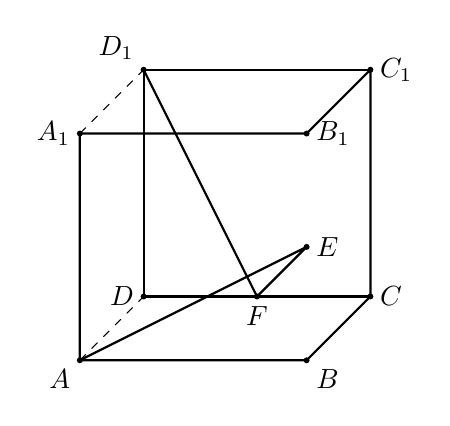
\begin{tikzpicture}[scale=0.9, >=stealth]
  \coordinate (A)  at (0,0);
  \coordinate (B)  at (3.2,0);
  \coordinate (C)  at (4.1,0.9);
  \coordinate (D)  at (0.9,0.9);
  \coordinate (A1) at (0,3.2);
  \coordinate (B1) at (3.2,3.2);
  \coordinate (C1) at (4.1,4.1);
  \coordinate (D1) at (0.9,4.1);
  \coordinate (E)  at (3.2,1.6);
  \coordinate (F)  at (2.5,0.9);

  \draw[thick] (A)--(B)--(C)--(C1)--(B1)--(A1)--cycle;
  \draw[thick] (D)--(C) (D)--(D1) (D1)--(C1);
  \draw[dashed] (A)--(D) (A1)--(D1);
  \draw[thick] (A)--(E) (E)--(F) (D1)--(F);

  \fill (A)  circle (1.2pt) node[below left] {$A$};
  \fill (B)  circle (1.2pt) node[below right] {$B$};
  \fill (C)  circle (1.2pt) node[right] {$C$};
  \fill (D)  circle (1.2pt) node[left] {$D$};
  \fill (A1) circle (1.2pt) node[left] {$A_1$};
  \fill (B1) circle (1.2pt) node[right] {$B_1$};
  \fill (C1) circle (1.2pt) node[right] {$C_1$};
  \fill (D1) circle (1.2pt) node[above left] {$D_1$};
  \fill (E)  circle (1.2pt) node[right] {$E$};
  \fill (F)  circle (1.2pt) node[below] {$F$};
\end{tikzpicture}
\end{center}
\nopagebreak[4]
\Needspace{4\baselineskip}
\textbf{解析}

\Needspace{5\baselineskip}
取坐标

\nopagebreak[4]
\[
A(0,0,0),\quad B(2,0,0),\quad C(2,2,0),\quad D(0,2,0),
\]

\Needspace{5\baselineskip}
并令竖直方向为第三坐标轴，则

\nopagebreak[4]
\[
A_1(0,0,2),\quad D_1(0,2,2),\quad E(2,0,1),\quad F(1,2,0).
\]

\gksubpart{(1)}

\Needspace{5\baselineskip}
有

\nopagebreak[4]
\[
\overrightarrow{AD}=(0,2,0),
\qquad
\overrightarrow{D_1F}=(1,0,-2),
\]

两向量内积为 $0$，故 $AD\perp D_1F$。

\gksubpart{(2)}

\Needspace{5\baselineskip}
又

\nopagebreak[4]
\[
\overrightarrow{AE}=(2,0,1),
\]

\Needspace{5\baselineskip}
且

\nopagebreak[4]
\[
\overrightarrow{AE}\cdot\overrightarrow{D_1F}=2-2=0.
\]

所以 $AE$ 与 $D_1F$ 所成的角为 $\pi/2$。

\gksubpart{(3)}

\Needspace{5\baselineskip}
直线 $D_1F$ 位于平面 $A_1FD_1$ 内，并且由前两问

\nopagebreak[4]
\[
D_1F\perp AD,\qquad D_1F\perp AE.
\]

由于 $AD$、$AE$ 是平面 $AED$ 内相交的两条直线，故 $D_1F\perp$ 平面 $AED$。因此平面 $AED$ 与平面 $A_1FD_1$ 垂直。

\gksubpart{(4)}

\Needspace{5\baselineskip}
三角形 $A_1D_1F$ 在 $D_1$ 处为直角，且

\nopagebreak[4]
\[
A_1D_1=2,\qquad D_1F=\sqrt5,
\]

\Needspace{5\baselineskip}
所以

\nopagebreak[4]
\[
S_{\triangle A_1D_1F}=\frac12\times2\times\sqrt5=\sqrt5.
\]

\Needspace{5\baselineskip}
平面 $A_1D_1F$ 的方程为 $2x+z=2$，点 $E(2,0,1)$ 到该平面的距离为

\nopagebreak[4]
\[
h=\frac{|2\times2+1-2|}{\sqrt{2^2+1^2}}=\frac3{\sqrt5}.
\]

\Needspace{5\baselineskip}
故

\nopagebreak[4]
\[
V_{F-A_1ED_1}
=\frac13\,S_{\triangle A_1D_1F}\,h
=\frac13\times\sqrt5\times\frac3{\sqrt5}=1.
\]

\gkanswer{答案（1）：见解析版}

\gkanswer{答案（2）：$\dfrac\pi2$}

\gkanswer{答案（3）：见解析版}

\gkanswer{答案（4）：$1$}

\end{answer}
\begin{answer}
\gksolhead{24}{}

\textbf{题目}：

设二次函数 $f(x)=ax^2+bx+c\ (a>0)$，方程 $f(x)-x=0$ 的两个根 $x_1,x_2$ 满足 $0<x_1<x_2<\dfrac1a$。

（1） 当 $x\in(0,x_1)$ 时，证明 $x<f(x)<x_1$；

（2） 设函数 $f(x)$ 的图象关于直线 $x=x_0$ 对称，证明 $x_0<\dfrac{x_1}{2}$。

\Needspace{4\baselineskip}
\textbf{解析}

\gksubpart{(1)}

\Needspace{5\baselineskip}
令

\nopagebreak[4]
\[
g(x)=f(x)-x=a(x-x_1)(x-x_2).
\]

\Needspace{5\baselineskip}
当 $0<x<x_1$ 时，$x-x_1<0$ 且 $x-x_2<0$，所以 $g(x)>0$，从而

\nopagebreak[4]
\[
f(x)>x.
\]

\Needspace{5\baselineskip}
令 $t=x_1-x>0$，则 $x_2-x<x_2<1/a$，并且

\nopagebreak[4]
\[
f(x)=x+a(x_1-x)(x_2-x)
=x_1-t+a,t(x_2-x)
=x_1-t\bigl(1-a(x_2-x)\bigr)<x_1.
\]

于是 $x<f(x)<x_1$。

\gksubpart{(2)}

\Needspace{5\baselineskip}
方程 $f(x)-x=0$ 写成

\nopagebreak[4]
\[
ax^2+(b-1)x+c=0.
\]

\Needspace{5\baselineskip}
由韦达定理

\nopagebreak[4]
\[
x_1+x_2=\frac{1-b}{a}.
\]

\Needspace{5\baselineskip}
抛物线 $f(x)$ 的对称轴为 $x=x_0$，其中

\nopagebreak[4]
\[
x_0=-\frac b{2a}
=\frac{x_1+x_2}{2}-\frac1{2a}.
\]

\Needspace{5\baselineskip}
由于 $x_2<1/a$，有 $1/(2a)>x_2/2$，因此

\nopagebreak[4]
\[
x_0<\frac{x_1+x_2}{2}-\frac{x_2}{2}=\frac{x_1}{2}.
\]

\gkanswer{答案（1）：见解析版}

\gkanswer{答案（2）：见解析版}

\end{answer}
\begin{answer}
\gksolhead{25}{}

\textbf{题目}：

设圆满足：①截 $y$ 轴所得弦长为 2；②被 $x$ 轴分成两段圆弧，其弧长的比为 $3:1$。在满足条件①、②的所有圆中，求圆心到直线 $l:x-2y=0$ 的距离最小的圆的方程。

\Needspace{4\baselineskip}
\textbf{解析}

\Needspace{5\baselineskip}
设圆心为 $(u,v)$，半径为 $r$。圆截 $y$ 轴所得弦长为 $2$，所以

\nopagebreak[4]
\[
2\sqrt{r^2-u^2}=2,qquad r^2-u^2=1.
\]

\Needspace{5\baselineskip}
$x$ 轴把圆分成弧长比为 $3:1$ 的两段，因此对应的圆心角为 $3\pi/2$ 和 $\pi/2$。弦到圆心的距离为 $r\cos(\pi/4)=r/\sqrt2$，即

\nopagebreak[4]
\[
r^2=2v^2.
\]

\Needspace{5\baselineskip}
联立得

\nopagebreak[4]
\[
2v^2=1+u^2.
\]

\Needspace{5\baselineskip}
圆心到直线 $l:x-2y=0$ 的距离满足

\nopagebreak[4]
\[
d^2=\frac{(u-2v)^2}{5}.
\]

\Needspace{5\baselineskip}
由 $(u-v)^2\geqslant0$ 得 $u^2+v^2\geqslant2uv$，所以

\nopagebreak[4]
\[
(u-2v)^2
=u^2-4uv+4v^2
\geqslant u^2+4v^2-2u^2-2v^2
=2v^2-u^2=1.
\]

\Needspace{5\baselineskip}
等号成立当且仅当 $u=v$。代入 $2v^2=1+u^2$ 得 $u=v=1$ 或 $u=v=-1$，同时 $r^2=2$。因此所求圆为

\nopagebreak[4]
\[
(x-1)^2+(y-1)^2=2
\]

\Needspace{5\baselineskip}
或

\nopagebreak[4]
\[
(x+1)^2+(y+1)^2=2.
\]

\gkanswer{答案：$(x-1)^2+(y-1)^2=2$ 或 $(x+1)^2+(y+1)^2=2$}

\end{answer}